\documentclass[a4paper, 12pt]{report}

\usepackage[dvipsnames]{xcolor}

%%%%%%%%%%%%%%%%
% Set Variables %
%%%%%%%%%%%%%%%%

\def\useItalian{0}  % 1 = Italian, 0 = English

\def\courseName{Advanced Algorithms}

\def\coursePrerequisites{\begin{itemize} \item Progettazione degli Algoritmi \end{itemize}}

\def\book{TODO}

% \def\authorName{Simone Bianco}
% \def\email{bianco.simone@outlook.it}
% \def\github{https://github.com/Exyss/university-notes}
% \def\linkedin{https://www.linkedin.com/in/simone-bianco}

\def\authorName{Alessio Bandiera}
\def\email{alessio.bandiera02@gmail.com}
\def\github{https://github.com/aflaag-notes}
\def\linkedin{https://www.linkedin.com/in/alessio-bandiera-a53767223}

%%%%%%%%%%%%
% Packages %
%%%%%%%%%%%%

\usepackage{../../packages/Nyx/nyx-packages}
\usepackage{../../packages/Nyx/nyx-styles}
\usepackage{../../packages/Nyx/nyx-frames}
\usepackage{../../packages/Nyx/nyx-macros}
\usepackage{../../packages/Nyx/nyx-title}
\usepackage{../../packages/Nyx/nyx-intro}

%%%%%%%%%%%%%%
% Title-page %
%%%%%%%%%%%%%%

\logo{../../packages/Nyx/logo.png}

\if\useItalian1
    \institute{\curlyquotes{\hspace{0.25mm}Sapienza} Università di Roma}
    \faculty{Ingegneria dell'Informazione,\\Informatica e Statistica}
    \department{Dipartimento di Informatica}
    \ifdefined\book
        \subtitle{Appunti integrati con il libro \book}
    \fi
    \author{\textit{Autore}\\\authorName}
\else
    \institute{\curlyquotes{\hspace{0.25mm}Sapienza} University of Rome}
    \faculty{Faculty of Information Engineering,\\Informatics and Statistics}
    \department{Department of Computer Science}
    \ifdefined\book
        \subtitle{Lecture notes integrated with the book \book}
    \fi
    \author{\textit{Author}\\\authorName}
\fi


\title{\courseName}
\date{\today}

% \supervisor{Linus \textsc{Torvalds}}
% \context{Well, I was bored\ldots}

\addbibresource{./references.bib}

%%%%%%%%%%%%
% Document %
%%%%%%%%%%%%

\begin{document}
    \maketitle

    % The following style changes are valid only inside this scope 
    {
        \hypersetup{allcolors=black}
        \fancypagestyle{plain}{%
        \fancyhead{}        % clear all header fields
        \fancyfoot{}        % clear all header fields
        \fancyfoot[C]{\thepage}
        \renewcommand{\headrulewidth}{0pt}
        \renewcommand{\footrulewidth}{0pt}}

        \romantableofcontents
    }

    \introduction

    %%%%%%%%%%%%%%%%%%%%%

    \chapter{TODO}

    placeholder \todo{missing introduction}

    \section{TODO}

    \subsection{The Max Cut problem}

    The first problem that will be discussed is the \href{https://en.wikipedia.org/wiki/Maximum_cut}{Maximum Cut} problem (or \tit{Max Cut}, for short). The \tbf{Max Cut problem} --- in the unweighted case --- is a classic combinatorial optimization problem in the branch of \href{https://en.wikipedia.org/wiki/Graph_theory}{graph theory}, in which we seek to partition the vertices of an undirected graph into two disjoint subsets while maximizing the number of edges that have endpoints in both subsets. More formally, we will define a \tbf{cut} of a graph as follows.

    \begin{frameddefn}{Cut}
        Given an undirected graph $G = (V, E)$, and a subset of its vertices $S \subseteq V$, the \tbf{cut} induced by $S$ on $G$ is defined as follows $$\mathrm{cut}(S) := \{e \in E \quad \abs{S \cap e} = 1\}$$
    \end{frameddefn}

    Note that in the definition above we are defining the cut of a graph through the intersection between a set of vertices $S$ and edges in $E$; this is because, in the undirected case, we will consider the edges of a graph $G = (V, E)$ as sets of 2 elements $$E = \{\{u, v\} \quad u, v \in V\}$$ Therefore, given a set of vertices $S$, the cut induced by $S$ is simply the set of edges that have only one endpoint in $S$ (implying that the other one will be in $V - S$).

    \begin{figure}[H]
        \centering
        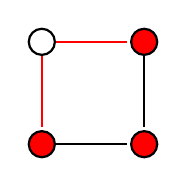
\begin{tikzpicture}[-,>=stealth,shorten >=1pt,auto,node distance=1.3cm, thick,main node/.style={scale=0.9,circle,draw,font=\sffamily\normalsize}]

            \node[circle, draw]  (1) []{};
            \node[circle, draw, fill=red]  (2) [below of = 1]{};
            \node[circle, draw, fill=red]  (3) [right of = 1]{};
            \node[circle, draw, fill=red]  (4) [below of = 3]{};

            % \path[every node/.style={font=\sffamily\small}]

            \draw[-] (1) [red] to (2);
            \draw[-] (1) [red] to (3);
            \draw[-] (2) to (4);
            \draw[-] (3) to (4);

            ;
        \end{tikzpicture}
        \caption{Given the set of red vertices $S$, the green edges represent $\mathrm{cut}(S)$.}
    \end{figure}

    With this definition, we can introduce the \tbf{Max Cut} problem, which is defined as follows.

    \begin{frameddefn}{Max Cut problem}
        The \tbf{Max Cut} (MC) problem is defined as follows: iven an undirected graph $G = (V, E)$, determine the set $S \subseteq V$ that maximizes $\abs{\mathrm{cut}(S)}$.
    \end{frameddefn}

    Although this problem is known to be \textsf{APX-Hard} \cite{maxcut}, approximation algorithms and heuristic methods like greedy algorithms and local search are commonly used to find near-optimal solutions.

    For now, we present the following \tbf{randomized algorithm}, which provides a straightforward $\frac{1}{2}$-approximation for MC. This algorithm runs in polynomial time and achieves the approximation guarantee with high probability.

    \begin{framedalgo}{Random Cut}
        Given an undirected graph $G = (V, E)$, the algorithm returns a cut of $G$. \\
        \hrule

        \quad
        \begin{algorithmic}[1]
            \Function{RandomCut}{$G$}
                \State $S := \varnothing$
                \For{$v \in V$}
                    \State Let $c_v$ be the outcome of the flip of an independent fair coin
                    \If{$c_v == \mathrm H$}
                        \State $S = S \cup \{v\}$
                    \EndIf
                \EndFor
                \State \textbf{return} $S$
            \EndFunction
        \end{algorithmic}
    \end{framedalgo}

    Note that this algorithm is powerful, because \tit{it does not care about the structure of the graph in input}, since the output is completely determined by the coin flips performed in the \texttt{for} loop. Now we will prove that this algorithm provides a correct \tbf{expected $\frac{1}{2}$-approximation} of MC.
    
    \begin{framedthm}[label={expected random cut}]{Expected approximation ratio of \textsc{RandomCut}}
        Let $G= (V, E)$ be a graph, and let $S^*$ be an optimal solution to MC on $G$. Then, given $S = \textsc{RandomCut}(G)$, it holds that $$\mathbb E [\abs{\mathrm{cut}(S)}] \ge \dfrac{\abs{\mathrm{cut}(S^*)}}{2}$$
    \end{framedthm}

    \begin{proof}
        By definition, note that $$\forall e \in E \quad e \in \mathrm{cut}(S) \iff \abs{S \cap e} = 1$$ Consider an edge $e = \{v, w\} \in E$; then, by definition $$\{v, w\} \in \mathrm{cut}(S) \iff (v \in S \land w \notin S) \lor (v \notin S \land w \in S)$$ and let $\xi_1$ and $\xi_2$ be these last two events respectively. Then $$\Pr[\xi_1] = \Pr[c_v = \mathrm{heads} \land c_w = \mathrm{tails}]$$ by definition of the algorithm, and by independence of the flips of the fair coins we have that $$\Pr[\xi_1] = \Pr[c_v = \mathrm{heads}] \cdot \Pr[c_w = \mathrm{tails}] = \dfrac{1}{2} \cdot \dfrac{1}{2} = \dfrac{1}{4}$$ Analogously, we can show that $$\Pr[\xi_2] = \dfrac{1}{4}$$ This implies that $$\Pr[e \in \mathrm{cut}(S)] = \Pr[\xi_1 \lor \xi_2] = \Pr[\xi_1] + \Pr[\xi_2] - \Pr[\xi_1 \land \xi_2] = \dfrac{1}{4} + \dfrac{1}{4} - 0 = \dfrac{1}{2}$$ Hence, we have that $$\mathbb E [\abs{\mathrm{cut}(S)}] = \sum_{e \in E}{1 \cdot \Pr[e \in \mathrm{cut}(S)]} = \dfrac{\abs E}{2} \ge \dfrac{\abs{\mathrm{cut}(S^*)}}{2}$$ where the last inequality directly follows from the definition of cut of a graph.
    \end{proof}

    As previously mentioned, this algorithm has an \tbf{expected approximation ratio} of $\frac{1}{2}$, which implies that it may return very bad solutions in some cases, depending on the outcomes of the coin flips. However, thanks to the following algorithm, we can actually transform the \tbf{guarantee of expectations} into a \tbf{guarantee of high probability} --- note that it is possible to show that the previous algorithm provides guarantee of high probability as well, but the proof is much more complex.

    \begin{framedalgo}{$t$-times Random Cut}
        Given an undirected graph $G = (V, E)$ and an integer $t > 0$, the algorithm returns a cut of $G$. \\
        \hrule

        \quad
        \begin{algorithmic}[1]
            \Function{$t$-timesRandomCut}{$G$, $t$}
                \For{$i \in [t]$}
                    \State $S_i := \textsc{RandomCut}(G)$
                \EndFor
                \State \textbf{return} $S \in \argmax_{i \in [t]}{\abs{\mathrm{cut}(S_i)}}$
            \EndFunction
        \end{algorithmic}
    \end{framedalgo}

    The algorithm above simply runs the \textsc{RandomCut} algorithm $t$ times, and returns the set $S_i$ that maximizes the cut, among all the various $S_1, \ldots, S_t$. The following theorem will show that a \tit{reasonable number} of runs of the \textsc{RandomCut} algorithm suffices in order to almost certainly obtain a $\approx \frac{1}{2}$-approximation of any optimal solution.

    \begin{framedthm}{}
        Let $G= (V, E)$ be a graph, and let $S^*$ be an optimal solution to MC on $G$. Then, given $S = \textsc{$t$-timesRandomCut}(G, t)$, it holds that $$\Pr \sbk{\abs{\mathrm{cut}(S)} > \dfrac{1 - \varepsilon}{2} \abs{\mathrm{cut}(S^*)}} > 1 - \delta$$ where $t = \frac{2}{\varepsilon} \ln {\frac{1}{\delta}}$ and $0 < \varepsilon, \delta < 1$.
    \end{framedthm}
    
    \begin{proof}
        For each $i \in [t]$, let $C_i := \abs{\mathrm{cut}(S_i)}$ for each $S_i$ defined by the algorithm, and let $N_i := \abs E - C_i$. Let $0 < \varepsilon < 1$; since $N_i$ is a non-negative random variable, by \href{https://en.wikipedia.org/wiki/Markov%27s_inequality}{Markov's inequality} we have that $$\Pr[N_i \ge (1 + \varepsilon) \mathbb E [N_i]] \le \dfrac{1}{1 + \varepsilon} = 1 - \dfrac{\varepsilon}{1 + \varepsilon} \le 1 - \dfrac{\varepsilon}{2}$$ In particular, this inequality can be rewritten as follows:
        \begin{equation*}
            \begin{split}
                1 - \dfrac{\varepsilon}{2} &\ge \Pr[N_i \ge (1 + \varepsilon) \mathbb E [N_i]] \\
                                           &= \Pr[\abs E - C_i \ge (1 + \varepsilon)(\abs E - \mathbb E [C_i])] \\
                                           &= \Pr[- \varepsilon \abs E \ge C_i - (1 + \varepsilon) \mathbb E [C_i]]
            \end{split}
        \end{equation*}
        As shown in the proof of \cref{expected random cut}, we know that $\mathbb E [C_i] = \frac{\abs E}{2}$, therefore
        \begin{equation*}
            \begin{split}
                1 - \dfrac{\varepsilon}{2} &\ge \Pr[- \varepsilon \abs E \ge C_i - (1 + \varepsilon) \mathbb E [C_i]] \\
                                           &= \Pr \sbk{- \varepsilon \abs E \ge C_i - \dfrac{1 + \varepsilon}{2} \abs E} \\
                                           &= \Pr \sbk{- \varepsilon \dfrac{\abs E}{2} \ge C_i - \dfrac{\abs E}{2}} \\
                                           &= \Pr \sbk{\dfrac{1 - \varepsilon}{2} \abs E\ge C_i} \\
                                           &= \Pr \sbk{(1 - \varepsilon) \mathbb E[C_i] \ge C_i} \\
            \end{split}
        \end{equation*}
        Note that the event in the last probability, namely $$\abs{\mathrm{cut}(S_i)}  \le (1 - \varepsilon) \mathbb E [\abs{\mathrm{cut}(S_i)}]$$ corresponds to a \curlyquotes{bad} solution, i.e. one whose cardinality is at most $(1 - \varepsilon)$-th of the expected value.

        By definition of the algorithm, each of the $t$ runs of the \textsc{RandomCut} algorithm is independent from the others, therefore the probability of \tit{all} the solutions $S_1, \ldots, S_t$ being \curlyquotes{bad} is bounded by $$\Pr[\forall i \in [t]  \quad C_i \le (1 - \varepsilon) \mathbb E [C_i]] = \prod_{i = 1}^t{\Pr[C_i \le (1 - \varepsilon)\mathbb E[C_i]]} \le \rbk{1 - \dfrac{\varepsilon}{2}}^t$$

        Using the fact that $$\forall x \in \R \quad 1 - x \le e^{-x} \implies 1 - \frac{\varepsilon}{2} \le e^{- \frac{\varepsilon}{2}}$$ we have that $$\Pr[\forall i \in [t] \quad C_i \le (1 - \varepsilon) \mathbb E[C_i]] \le \rbk{1 - \dfrac{\varepsilon}{2}}^t \le e^{- \frac{\varepsilon}{2} \cdot t} = e^{- \ln {\frac{1}{\delta}}} = \delta$$

        Therefore, the probability that at least one among $S_1, \ldots, S_t$ is a \curlyquotes{good} solution is bounded by $$\Pr[\exists i \in [t] \quad C_i > (1 - \varepsilon) \mathbb E [C_i]] = 1 - \Pr[\forall i \in [t] \quad C_i \le (1 - \varepsilon) \mathbb E [C_i]] \ge 1 - \delta$$

        placeholder \todo{last part}
    \end{proof}

    Note that this result is \tit{very powerful}: for instance, if $\varepsilon = \delta = 0.1$, we get that $$\Pr[\abs{\mathrm{cut}(S)} > 0.45 \cdot \abs{\mathrm{cut}(S^*)}] \ge 0.9$$ and $t \approx 46$, meaning that we just need to run the \textsc{RandomCut} algorithm approximately 46 times in order to get a solution that is better than a $0.45$-approximation with $90\%$ probability.

    \subsection{The Vertex Cover problem}

    Another very important problem in graph theory is the \href{https://en.wikipedia.org/wiki/Vertex_cover}{Vertex Cover} problem, which concerns the combinatorial structure of the \tbf{vertex cover}, defined as follows.

    \begin{frameddefn}{Vertex cover}
        Given an undirected graph $G = (V, E)$, a \tbf{vertex cover} of $G$ is a set of vertices $S \subseteq V$ such that $$\forall e \in E \quad \exists v \in S \quad v \in e$$
    \end{frameddefn}

    \begin{figure}[H]
        \centering
        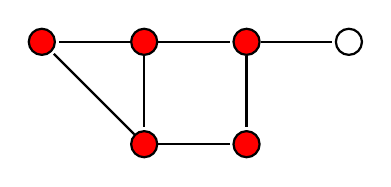
\begin{tikzpicture}[-,>=stealth,shorten >=1pt,auto,node distance=1.3cm, thick,main node/.style={scale=0.9,circle,draw,font=\sffamily\normalsize}]

            \node[circle, draw, fill=red] (1) []{};
            \node[circle, draw, fill=red] (2) [right of = 1]{};
            \node[circle, draw, fill=red] (3) [below of = 1]{};
            \node[circle, draw, fill=red] (4) [below of = 2]{};
            \node[circle, draw, fill=red] (5) [left of = 1]{};
            \node[circle, draw, ] (6) [right of = 2]{};

            \draw[-] (1) to (2);
            \draw[-] (1) to (3);
            \draw[-] (2) to (4);
            \draw[-] (1) to (5);
            \draw[-] (3) to (4);
            \draw[-] (3) to (5);
            \draw[-] (2) to (6);

            ;
        \end{tikzpicture}
        \caption{An example of a vertex cover.}
    \end{figure}

    As shown in figure, a vertex cover is simply a set of vertices that must \tit{cover} all the edges of the graph. Clearly, the trivial vertex cover is representd by $S = V$, but a more interesting solution to the problem is represented by the \tbf{minimum vertex cover}.

    \begin{frameddefn}{Vertex Cover problem}
        The \tbf{Vertex Cover} (VC) problem is defined as follows: given an undirected graph $G = (V, E)$, determine the vertex cover $S \subseteq V$ of smallest cardinality.
    \end{frameddefn}

    \begin{figure}[H]
        \centering
        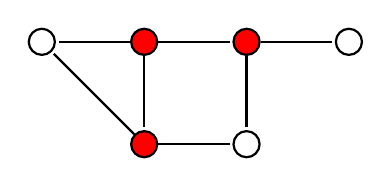
\begin{tikzpicture}[-,>=stealth,shorten >=1pt,auto,node distance=1.3cm, thick,main node/.style={scale=0.9,circle,draw,font=\sffamily\normalsize}]

            \node[circle, draw, fill=red] (1) []{};
            \node[circle, draw, fill=red] (2) [right of = 1]{};
            \node[circle, draw, fill=red] (3) [below of = 1]{};
            \node[circle, draw, ] (4) [below of = 2]{};
            \node[circle, draw, ] (5) [left of = 1]{};
            \node[circle, draw, ] (6) [right of = 2]{};

            \draw[-] (1) to (2);
            \draw[-] (1) to (3);
            \draw[-] (2) to (4);
            \draw[-] (1) to (5);
            \draw[-] (3) to (4);
            \draw[-] (3) to (5);
            \draw[-] (2) to (6);

            ;
        \end{tikzpicture}
        \caption{This is the \tit{minimum vertex cover} of the previous graph.}
    \end{figure}

    As famously proved by \textcite{karp} in 1972, this problem is \NPComplete, hence we are interested in finding algorithms that allow to find approximations of optimal solutions. For instance, an algorithm that is able to approximate VC concerns the \href{https://en.wikipedia.org/wiki/Matching_(graph_theory)}{matching} problem.

    \begin{frameddefn}{Matching}
        Given an undirected graph $G = (V, E)$, a \tbf{matching} of $G$ is a set of edges $A \subseteq E$ such that $$\forall e, e' \in A \quad e \cap e' = \varnothing$$
    \end{frameddefn}

    \begin{figure}[H]
        \centering
        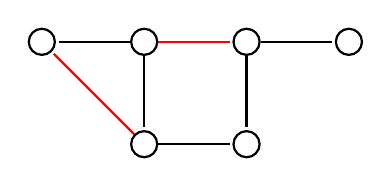
\begin{tikzpicture}[-,>=stealth,shorten >=1pt,auto,node distance=1.3cm, thick,main node/.style={scale=0.9,circle,draw,font=\sffamily\normalsize}]

            \node[circle, draw] (1) []{};
            \node[circle, draw] (2) [right of = 1]{};
            \node[circle, draw] (3) [below of = 1]{};
            \node[circle, draw] (4) [below of = 2]{};
            \node[circle, draw] (5) [left of = 1]{};
            \node[circle, draw] (6) [right of = 2]{};

            \draw[-] (1) [red] to (2);
            \draw[-] (1) to (3);
            \draw[-] (2) to (4);
            \draw[-] (1) to (5);
            \draw[-] (3) to (4);
            \draw[-] (3) [red] to (5);
            \draw[-] (2) to (6);

            ;
        \end{tikzpicture}
        \caption{A \tit{matching} of the previous graph.}
        \label{matching}
    \end{figure}

    As shown in figure, a matching is nothing more than a set of edges that must not share endpoints with each other --- for this reason, in literature it is often referred to as \tbf{independent edge set}. Differently from the vertex cover structure, in this context the trivial matching is clearly the set $A = \varnothing$, which vacuously satisfies the matching condition. However, a more interesting solution is represented by the \tbf{maximum matching}, but this time we have to distinguish two slightly different definitions, namely the concept of \tit{maximal} and \tit{maximum}.

    \begin{frameddefn}{Maximal matching}
        A \tbf{maximal matching} is a matching that cannot be extended any further.
    \end{frameddefn}
    
    For instance, the matching shown in \cref{matching} is actually a \tbf{maximal matching}, because no other edge in $E$ can be added to the current set of edges $A$ of the matching without breaking the matching condition.

    \begin{frameddefn}{Maximum matching}
        A \tbf{maximum matching} is a matching that has the largest cardinality.
    \end{frameddefn}
    
    Clearly, the previous example does not represent a \tbf{maximum matching}, because the following set of edges

    \begin{figure}[H]
        \centering
        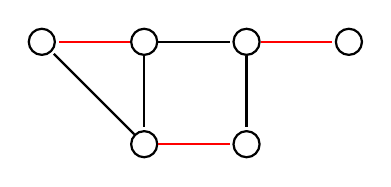
\begin{tikzpicture}[-,>=stealth,shorten >=1pt,auto,node distance=1.3cm, thick,main node/.style={scale=0.9,circle,draw,font=\sffamily\normalsize}]

            \node[circle, draw] (1) []{};
            \node[circle, draw] (2) [right of = 1]{};
            \node[circle, draw] (3) [below of = 1]{};
            \node[circle, draw] (4) [below of = 2]{};
            \node[circle, draw] (5) [left of = 1]{};
            \node[circle, draw] (6) [right of = 2]{};

            \draw[-] (1) to (2);
            \draw[-] (1) to (3);
            \draw[-] (2) to (4);
            \draw[-] (1) [red] to (5);
            \draw[-] (3) [red] to (4);
            \draw[-] (3) to (5);
            \draw[-] (2) [red] to (6);

            ;
        \end{tikzpicture}
    \end{figure}

    is still a valid matching for the graph, but has a larger cardinality than the previous set.

    Differently from VC, a \tit{maximum matching} can be found in polynomial time. Moreover, the following algorithm can be used to determine a \tit{maximal matching} of a given graph.

    \begin{framedalgo}{Maximal matching}
        Given an undirected graph $G = (V, E)$, the algorithm returns a maximal matching of $G$. \\
        \hrule

        \quad
        \begin{algorithmic}[1]
            \Function{MaximalMatching}{$G$}
                \State $S := \varnothing$
                \While{$E \neq \varnothing$}
                    \State Choose $e\in E$
                    \State $S = S \cup \{e\}$
                    \State Remove from $E$ all the edges incident on $u$ or on $v$
                    \State $E = E - \{e\}$
                \EndWhile
                \State \textbf{return} $S$
            \EndFunction
        \end{algorithmic}
    \end{framedalgo}

    \idea{
        The algorithm is very straightforward: at each iteration, a random edge $e = \{u, v\}$ is chosen from $E$, and then any edge $e' \in E$ such that $e \cap e' \neq \varnothing$ is removed from $E$.

        Clearly, line 6 ensures that the output is a \tit{matching}, and the terminating condition of the \texttt{while} loop ensures that it is \tit{maximal}, but since the output depends on the chosen edges, $S$ is not guaranteed to be \tit{maximum}.
    }

    Another major reason on why we focus on matchings is the following theorem.

    \begin{framedthm}{Matchings bound vertex covers}
        Given an undirected graph $G = (V, E)$, a matching $A \subseteq E$ of $G$, and a vertex cover $S \subseteq V$ of $G$, we have that $\abs S \ge \abs A$.
    \end{framedthm}

    \begin{proof}
        By definition, any vertex cover $S$ of $G = (V, E)$ is also a vertex cover for $G^B = (V, B)$, for any set of edges $B \subseteq E$, and in particular this is true for $G^A = (V, A)$.

        Now consider $G^A$, and a vertex cover $C$ on it: by construction we have that $\Delta \le 1$, therefore any vertex in $C$ will cover at most 1 edge of $A$. This implies that if $\abs C = k$, then $C$ will cover at most $k$ edges of $G^A$.

        Lastly, since $G^A$ has $\abs A$ edges by definition, any vertex cover defined on $G^A$ has to contain at least $\abs A$ vertices. This implies that no vertex cover $S$ of $G$ smaller than $\abs A$ can exist, because $S$ will have to cover at least the edges in $A$.
    \end{proof}
    
    Thanks to this theorem, we can easily show that the algorithm that we just presented in order to find maximal matchings is a 2-approximation of VC. 

    \begin{framedthm}{2-approximation of VC problem}
        Given a graph $G$, and $M = \textsc{MaximalMatching}(G)$, let $S := \bigcup_{e \in M}{e}$. Then $S$ is a 2-approximation of VC on $G$.
    \end{framedthm}

    \begin{proof}
        Consider an optimal solution $S^*$ to VC on $G$, and let $M = \{e_1, \ldots, e_t\}$. Note that at each iteration of the algorithm exactly 1 edge is added to $M \subseteq V$, hence it always holds that $$S_i \cap S_{i + 1} = e_i = \{u, v\}$$ for any iteration $i \in [t - 1]$. Moreover, since $M$ is a matching, it holds that $\forall e, e' \in M \quad e \cap e' = \varnothing$, therefore $\abs{S} = 2 \abs{M}$. Finally, by the previous theorem we have that $\abs{M} \le \abs{S^*}$, concluding that $$\abs S = 2 \abs M \le 2 \abs{S^*}$$
    \end{proof}
    
    This 2-approximation algorithm is conjectured to be optimal, but it has not been proven yet. In fact, VC is conjectured to be \NPHard to $(2 - \varepsilon)$-approximate, for any $\varepsilon > 0$.

    Interestingly, the decisional version of VC is \href{https://en.wikipedia.org/wiki/Parameterized_complexity#FPT}{Fixed Parameter Tractable}. This characterization comes from the nature of the problem: for each edge $e = \{u, v\}$ of a given undirected graph $G = (V, E)$, either $u$ or $v$ has to be in the vertex cover, therefore it possible to approach VC by trying all possible choices of set of vertices $S \subseteq V$, and backtrack if necessary. The following algorithm employs this idea.

    \begin{framedalgo}{Decisional VC}
        Given an undirected graph $G = (V, E)$, and an integer $k$, the algorithm returns \texttt{True} if and only if $G$ admits a vertex cover of size $k$. \\
        \hrule

        \quad
        \begin{algorithmic}[1]
            \Function{VC}{$G$, $k$}
                \If{$E == \varnothing$}
                    \State \tbf{return} \texttt{True}
                \ElsIf{$k == 0$}
                    \State \tbf{return} \texttt{False}
                \Else
                    \State Choose $e = \{u, v\} \in E$
                    \If{$\textsc{VC}(G[V - \{u\}]), k - 1)$}
                        \State \tbf{return} \texttt{True}
                    \EndIf
                    \If{$\textsc{VC}(G[V - \{v\}]), k - 1)$}
                        \State \tbf{return} \texttt{True}
                    \EndIf
                    \State \tbf{return} \texttt{False}
                \EndIf
            \EndFunction
        \end{algorithmic}
    \end{framedalgo}

    Note that this algorithm actually solves the \tit{decisional} version of VC. Moreover, the algorithm uses the definition of \tbf{induced subgraph}, which is the following.

    \begin{frameddefn}{Induced subgraph}
        Given an undirected graph $G = (V, E)$, and a set of vertices $S \subseteq V$, then $G[S]$ represents the \tbf{subgraph induced by $S$ on $G$}, and it is obtained by removing from $G$ all the nodes of $V - S$ --- and their corresponding edges.
    \end{frameddefn}

     \begin{figure}[H]
        \centering

        \begin{tabular}{ccc}
            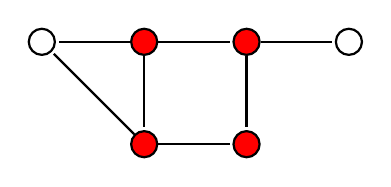
\begin{tikzpicture}[-,>=stealth,shorten >=1pt,auto,node distance=1.3cm, thick,main node/.style={scale=0.9,circle,draw,font=\sffamily\normalsize}]

                \node[circle, draw, fill=red] (1) []{};
                \node[circle, draw, fill=red] (2) [right of = 1]{};
                \node[circle, draw, fill=red] (3) [below of = 1]{};
                \node[circle, draw, fill=red] (4) [below of = 2]{};
                \node[circle, draw] (5) [left of = 1]{};
                \node[circle, draw] (6) [right of = 2]{};

                \draw[-] (1) to (2);
                \draw[-] (1) to (3);
                \draw[-] (2) to (4);
                \draw[-] (1) to (5);
                \draw[-] (3) to (4);
                \draw[-] (3) to (5);
                \draw[-] (2) to (6);

                ;
            \end{tikzpicture}

            &\qquad\qquad&

            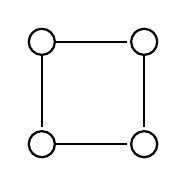
\begin{tikzpicture}[-,>=stealth,shorten >=1pt,auto,node distance=1.3cm, thick,main node/.style={scale=0.9,circle,draw,font=\sffamily\normalsize}]

                \node[circle, draw] (1) []{};
                \node[circle, draw] (2) [right of = 1]{};
                \node[circle, draw] (3) [below of = 1]{};
                \node[circle, draw] (4) [below of = 2]{};

                \draw[-] (1) to (2);
                \draw[-] (1) to (3);
                \draw[-] (2) to (4);
                \draw[-] (3) to (4);

                ;
            \end{tikzpicture}
        \end{tabular}

        \caption{On the left: a graph $G$ and a set of vertices $S$. On the right: the graph $G[S]$.}
    \end{figure}

    \idea{
        The structure of the algorithm consists of a simple backtracking algorithm:
        \begin{itemize}
            \item if the current graph has no edges, we covered every edge of the graph, therefore we return \texttt{True}
            \item if the current graph has some edges, but $k = 0$, then $G$ does not admit a vertex cover of size $k$, thus we return \texttt{False}
            \item if the current graph has some edges, and $k \neq 0$, then we choose an edge $e = \{u, v\} \in E$ arbitrarily, and we try to consider first $u$ then $v$ in a possible vertex cover --- note that $G[V - \{x\}]$ is a graph that does not contain $x$, neither any edge adjacent to it; if both attempts fail, we return \texttt{False}
        \end{itemize}
    }

    \cost{
        It is easy to see that the cost directly depends on the number of recursive calls that the algorithm performs, which is $2^k$ in the worst case, and the cost of constructing $G[V - \{x\}]$, which we can assume to be $O\rbk{n^2}$. Hence, the algorithm has a total cost of $O \rbk{2^k \cdot n^2}$.
    }

    \section{Mathematical Programming}

    Up to this point, we have introduced several \NPComplete problems and discussed approximation algorithms that provide near-optimal solutions within a certain approximation ratio. We will now explore a new technique that can be leveraged to design approximation algorithms for a broader class of problems, namely \tbf{mathematical programming}.

    \href{https://en.wikipedia.org/wiki/Mathematical_optimization}{Mathematical programming} is a powerful framework used to model and solve \tbf{optimization problems} across various fields, including operations research, computer science and engineering. It provides a structured way to \tit{maximize} or \tit{minimize} an \tbf{objective function} while satisfying a set of \tbf{constraints}. In particular, optimization problems are usually expressed as follows

    \begin{figure}[H]
        \centering
        \[\begin{array}{ccl}
            \qquad\qquad\quad
            & \max \; f(x) \\\\
            & g_i(x) \le b_i & \forall i \in [n] \\
            & x \in V
        \end{array}\]
    \end{figure}

    In this example, we see that

    \begin{itemize}
        \item $x$ is a \tit{vector} that lies inside the vector space $V$
        \item the objective function is $f(x)$, which can be either maximized or minimized
        \item $g_i(x) \le b_i$ is a constraint --- i.e. an inequality --- that $x$ must satisfy
    \end{itemize}

    Among the most widely studied forms of mathematical programming are \tbf{Linear Programming} (LP), \tbf{Integer Programming} (IP), and \tbf{Semidefinite Programming} (SDP), each with distinct properties and applications.

    Starting from linear programming, in LPs both the objective function and the constraints are \tit{linear} w.r.t. $V$, and there are no \tit{equality} constraints.

    \begin{figure}[H]
        \centering
        \[\begin{array}{ccl}
            \qquad\qquad\quad
            & \max \; x_1 + x_2 \\\\
            & 2x_1 + x_2 \le 10 \\
            & x_i \ge 0 & \forall i \in [n]\\
            & x \in \R^n
        \end{array}\]
        \caption{Example of an LP.}
    \end{figure}
   
    LPs can be solved in \tbf{polynomial time}: specifically, if an LP has $n$ variables, $m$ constraints, and each coefficient can be expressed as the ratio of two $t$-bit integers (where real numbers are approximated as rationals), then the \href{https://en.wikipedia.org/wiki/Ellipsoid_method}{Ellipsoid method} can solve it in time $O((nmt)^c)$ for some constant $c > 0$. This result extends, to some extent, to SDPs as well.

    Despite its theoretical guarantee of polynomial runtime, in practice the \href{https://en.wikipedia.org/wiki/Simplex_algorithm}{Simplex method} is often preferred, as it operates based on \tit{pivot rules}. In fact, although all known pivot rules for the Simplex method exhibit a theoretical \tit{exponential} lower bound due to specially constructed worst-case instances, its average performance is significantly better than that of the Ellipsoid method in real-world scenarios.

    \subsection{IPs and LP relaxation}

    Differently from LPs, in IPs the vector space of interest is $\{0, 1\}^n$. IPs can be used to solve a wide range of problems. For instance, given a graph $G =(V, E)$, the \tbf{vertex cover} problem that we discussed in the previous section can be formulated through the following IP:

    \begin{figure}[H]
        \centering
        \[\begin{array}{ccl}
            \qquad\qquad\quad
            & \min \; \displaystyle \sum_{u \in V}^n {x_v} \\\\
            & x_u + x_v \ge 1 & \forall \{u, v\} \in E \\
            & x_v \in \{0,1\} & \forall u \in V
        \end{array}\]
        \caption{IP for VC.}
    \end{figure}

    It is fairly straightforward to prove that an optimal solution to this IP yields an optimal solution to VC.

    \begin{framedlem}[label={vc ip}]{}
        Given a graph $G$, if $\{x^*_u\}_{u \in V}$ is an optimal solution to the previous IP, then $$S^* := \{v \in V \mid x^*_v = 1\}$$ is a minimum vertex cover for $G$.
    \end{framedlem}

    \begin{proof}
        Consider an optimal solution $\{x^*_u\}_{u \in V}$ to VC, and define $S^*$ as the set of vertices $v \in V$ such that $x^*_v = 1$. Note that any optimal solution is also a feasible solution, i.e. it satisfies the constraints of the IP.

        Note that the first constraint of the IP forces that for each $\{u, v\} \in E$ the sum between $x^*_u + x^*_v$ is at least one, and the second constraint forces each variable $x_v^*$ to be either 0 or 1. Therefore, together these two constraints imply that for any edge $\{u, v\} \in E$ at least one between $x_u^*$ and $x_v^*$ is 1, and by definition of $S^*$ this means at least one of the endpoints of $\{u, v\}$ is inside $S^*$. We conclude that $S^*$ is indeed a vertex cover for $G$, and by its definition note that $\abs{S^*} = \sum_{u \in V}{x^*_u}$.

        \claim{
            Given a vertex cover $S$ of a graph $G = (V, E)$, there exists a feasible solution $\{x_u\}_{u \in V}$ to the IP having value $\abs S$.
        }{
            Define the solution $\{x_u\}_{u \in V}$ by setting $x_u = 1$ if and only if $u \in S$. Clearly, the value of this solution is indeed $\sum_{u \in V}{x_u} = \abs S$; moreover, by definition of vertex cover, for any edge $\{u, v\} \in E$ at least one between $u$ and $v$ must be in $S$, therefore at least one between $x_u$ and $x_v$ is set to 1, implying that $x_u + x_v \ge 1$ is always satisfied.
        }

        By way of contradiction, suppose that $S^*$ is not a minimum vertex cover. Hence, there must exist another vertex cover $S'$ such that $\abs{S'} < \abs{S^*}$. By the previous claim, this implies that there exists a feasible solution $\{x'_u\}_{u \in V}$ for the IP that has value $\abs{S'}$, but then $$\sum_{u \in V}{x'_u} = \abs{S'} < \abs{S^*} = \sum_{u \in V}{x^*_u}$$ which contradicts the optimality of the solution of $\{x^*_u\}_{u \in V}$ for the IP.
    \end{proof}

    In particular, this lemma implies that VC can be reduced to Integer programming, indeed solving IPs is actually \NPHard \cite{karp}, differently from LPs. This result shows that IPs cannot be used \tit{directly} to obtain perfect solutions, but they are still very useful thanks to \tbf{relaxation}.

    To \tit{relax} an IP, we simply replace the constraint $x \in \{0, 1\}^n$ with $0 \le x \le 1$, transforming the IP into an LP.

    \begin{figure}[H]
        \centering
        \[\begin{array}{ccl}
            \qquad\qquad\quad
            & \min \; \displaystyle \sum_{u \in V}^n {x_v} \\\\
            & x_u + x_v \ge 1 & \forall \{u, v\} \in E \\
            & 0 \le x_v \le 1 & \forall u \in V
        \end{array}\]
        \caption{LP relaxation for the IP of VC.}
    \end{figure}

    But solving this LP is not enough to obtain a meaningful solution: in fact, a real-valued solution for this problem does not directly yield a vertex cover for a given graph. To fix this issue, the optimal solution of the LP relaxation is usually transformed through techniques such as \tbf{rounding}. Intuitively, the simplest possible type of \tit{rounding rule} is the following: given a solution $\{\overline x_u\}_{u \in V}$ to the LP relaxation, to obtain a VC consider the following set $$S := \cbk{v \in V \mid \overline x_v \ge \tfrac{1}{2}}$$ and for VC in particular, we can prove that this rounding rule actually yields a 2-approximation of any optimal solution.

    \begin{framedthm}[label={lp 2-approx vc}]{}
        Given a graph $G = (V, E)$, if $\{\overline x_u\}_{u \in V}$ is an optimal solution to the LP relaxation of the IP for VC, then $$\overline S := \cbk{v \in V \mid \overline x_v \ge \tfrac{1}{2}}$$ is a 2-approximation for VC.
    \end{framedthm}

    \begin{proof}
        Since $\{\overline x_u\}_{u \in V}$ is an optimal solution to the LP relaxation, it must satisfy the first constraint for which $\overline x_u + \overline x_v \ge 1$ for any $\{u, v\} \in E$. Moreover, for the second constraint we have that $\overline x_u \ge 0$ for all $u \in V$, therefore $$\forall \{u, v\} \in E \quad \max(\overline x_u, \overline x_v) \ge \dfrac{\overline x_u + \overline x_v}{2} \ge \dfrac{1}{2}$$ which means that at least one between $\overline x_u$ and $\overline x_v$ is at least $\frac{1}{2}$, implying that the edge $\{u, v\}$ will be covered by at least one of the two endpoints $u$ and $v$, by definition of $\overline S$. This proves that $\overline S$ is a vertex cover of $G$.

        To prove that $\overline S$ is indeed a 2-approximation, we just need to show the following: given a minimum vertex cover $S^*$ of $G$, it holds that $\abs{\overline S} \le 2 \abs{S^*}$. By the claim in \cref{vc ip}, we know that $S^*$ there exists a feasible solution $\{x^*_u\}_{u \in V}$ for the IP, which must be optimal for the IP since $S^*$ is a minimum vertex cover for $G$. Therefore, we have that
            \begin{equation*}
                \begin{split}
                    \abs{\overline S} &= \sum_{v \in \overline S}{1} \\
                                      &\le \sum_{v \in \overline S}{2 \overline x_v} \quad \quad \rbk{v \in \overline S \implies \overline x_v \ge \tfrac{1}{2}}\\
                                      &= 2 \sum_{v \in \overline S}{\overline x_v} \\
                                      &\le 2 \sum_{v \in V}{\overline x_v} \quad \quad \rbk{\overline S \subseteq V \land \overline x_v \ge 0} \\
                                      &\le 2 \sum_{v \in V}{x^*_v} \\
                                      &= 2 \abs{S^*}
                \end{split}
            \end{equation*}
            where the last inequality comes from the fact that the constraints of the LP are \tit{weaker} than the ones of the IP.
    \end{proof}

    However, note that this result should not come a surprise. In fact, consider a graph $G$, an optimal solution to the LP relaxation $\{\overline x_u\}_{u \in V}$ and $\overline S$ defined as previously shown; given an edge $\{u, v\} \in E(G)$, in the worst case we have that $$\overline x_u = \overline x_v = \dfrac{1}{2}$$ which still satisfies both constraints of the LP relaxation, since $\tfrac{1}{2} + \tfrac{1}{2} = 1 \ge 1$. This means that, in the worst case, both $u$ and $v$ end up inside $\overline S$, which gives an intuitive reason to why this LP relaxation indeed yields a 2-approximation solution.

    \subsection{Integrality gap}

    Consider a problem P, its equivalent IP, and the relative LP relaxation. Given an instance $I \in \mathrm P$ of the problem, we will denote with $\mathrm{IP^*_P}(I)$ and $\mathrm{LP^*_P}(I)$ the optimal values for the IP and the LP of the problem P on the instance $I$ --- we will omit P and $I$ the context is clear enough. Note that, in general, it holds that $\mathrm{LP^*} \le \mathrm{IP^*}$ since the constraints of the LP relaxation are \tit{weaker} than the ones of the IP.

    For example, the inequalities discussed in the proof of \cref{vc ip} could be rewritten as follows
    \begin{equation*}
        \begin{split}
            \abs{\overline S} &= \ldots \\
                              &\le 2 \sum_{v \in V}{\overline x_v} = 2 \mathrm{LP^*} \\
                              &\le 2 \sum_{v \in V}{x^*_v} = 2 \mathrm{IP^*} = 2 \abs{S^*}\\
        \end{split}
    \end{equation*}
    and in particular $\abs{\overline S} \le 2 \mathrm{LP^*} \le 2 \mathrm{IP^*}$. Can we improve this approximation ratio of 2 through LP relaxation? In general, for any $\alpha$ possible approximation ratio, it must hold that $$\alpha \ge \dfrac{\mathrm{IP^*}}{\mathrm{LP^*}}$$ because otherwise $$\alpha < \mathrm{\dfrac{IP^*}{LP^*}} \implies \abs{\overline S} \le \alpha \mathrm{LP^*} < \mathrm{\dfrac{IP^*}{LP^*}} \cdot \mathrm{LP^*} = \mathrm{IP^*}$$ meaning that $\overline S$ would be a solution better than the optimal solution of the IP, which is impossible. We can generalize this concept as follows.

    \begin{frameddefn}{Integrality gap}
        Given a problem P and an instance $I \in \mathrm P$, the \tbf{integrality gap} between $\mathrm{IP^*_P}(I)$ and $\mathrm{LP^*_P}(I)$ is defined as follows $$\mathrm{IG_P}(I) = \dfrac{\mathrm{IP^*_P}(I)}{\mathrm{LP^*_P}(I)}$$ The integrality gap for the problem P is defined as follows $$\mathrm{IG_P} = \sup_{I \in \mathrm P}{\mathrm{IG_P}(I)} = \sup_{I \in \mathrm P}{\dfrac{\mathrm{IP^*_P}(I)}{\mathrm{LP^*_P}(I)}}$$
    \end{frameddefn}

    In fact, through the previous argument, we can derive the following property that \tit{must} hold for any approximation ratio.

    \begin{framedprop}{Limits of LP relaxation}
        Given a problem P for which there is an $\alpha$-approximation algorithm which uses LP relaxation, it holds that

        \begin{itemize}
            \item if P is a \tbf{minimization problem}, then $\alpha \ge \mathrm{IG_P}$
            \item if P is a \tbf{maximixation problem}, then $\alpha \le \mathrm{IG_P}$
        \end{itemize}
    \end{framedprop}

    % This means that to improve this approximation ratio of 2, we would need to find a value $\varepsilon$ for which $$\abs{\overline S} \le (2 - \varepsilon) \mathrm{LP^*} \le (2 - \varepsilon) \mathrm{IP^*}$$

    Now, let us analyze again VC and try to bound $\mathrm{IG_{VC}}$. Consider the following \tit{clique} graph:
    
    \begin{figure}[H]
        \centering
        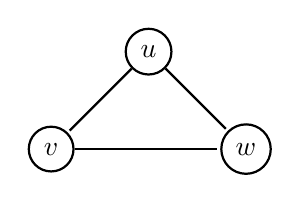
\begin{tikzpicture}[-,>=stealth,shorten >=1pt,auto,node distance=1.75cm, thick,main node/.style={scale=0.9,circle,draw,font=\sffamily\normalsize}]

            \node[circle, draw] (1) []{$u$};
            \node[circle, draw] (2) [below left of = 1]{$v$};
            \node[circle, draw] (3) [below right of = 1]{$w$};

            \draw[-] (1) to (2);
            \draw[-] (1) to (3);
            \draw[-] (2) to (3);

            ;
        \end{tikzpicture}
        \caption{The graph $K_3$.}
    \end{figure}

    it is easy to see that $$\mathrm{IP^*}(K_3) = 1 + 1 = 2$$ because 1 single node is not sufficient to cover all 3 edges in $E(K_3)$. However, since the values in the solution of the LP can be \tit{real-valued}, the value of an optimal solution for the LP relaxation is actually achieved by setting $$\overline x_u = \overline x_v = \overline x_w = \dfrac{1}{2} \implies \mathrm{LP}^*(K_3) = 3 \cdot \dfrac{1}{2} = \dfrac{3}{2}$$ therefore, by definition of IG we have that $$\exists I \in \mathrm P \quad \mathrm{IG_{VC}}(I) := \dfrac{\mathrm{IP^*_{VC}}(K_3)}{\mathrm{LP^*_{VC}}(K_3)} = \dfrac{2}{\tfrac{3}{2}} = \dfrac{4}{3} \implies \mathrm{IG_{VC}} := \sup_{I \in \mathrm P}{\dfrac{\mathrm{IP^*_{VC}}(I)}{\mathrm{LP^*_{VC}}(I)}} \ge \dfrac{4}{3}$$ 

    Moreover, \cref{lp 2-approx vc} shows that we already know an algorithm that employs LP relaxation which yields a 2-approximation of VC; therefore, this lower bound on $\mathrm{IG_{VC}}$ --- together with the previous proposition --- implies that any possible approximation ratio $\alpha$ on VC must satisfy $$2 \ge \alpha \ge \mathrm{IG_{VC}} \ge \dfrac{4}{3}$$ The following theorem proves that we can actually bound $\mathrm{IG_{VC}}$ tightly.

    \begin{framedthm}{Integrality gap for VC}
        $\mathrm{IG_{VC}} = 2$
    \end{framedthm}

    \begin{proof}
        We already proved that the upper bound is 2, so we just need to prove that the lower bound is 2 as well.

        Consider a clique $K_n$; by the same reasoning presented for the case of $K_3$, a feasible solution for the LP relaxation over this graph would be $$x_1 = \ldots = x_n = \dfrac{1}{2} \implies \mathrm{LP^*}(K_n) \le n \cdot \dfrac{1}{2} = \dfrac{n}{2}$$

        \claim{
            Any minimum vertex cover of $K_n$ has exactly $n - 1$ vertices.
        }{
            Consider a vertex cover $S = \{v_1\}$ for any vertex $v_1 \in V(K_n)$; since $K_n$ is a clique, by definition $\deg(v_1) = n - 1$, therefore $S$ is able to cover only $n - 1$ \tit{uncovered} edges of $K_n$. Now, consider another vertex $v_2 \in V(K_n)$, and add it to $S = \{v_1, v_2\}$; we observe that $\deg(v_2) = n - 1$, but $v_1 \sim v_2$ because $K_n$ is a clique, therefore $v_2$ will be able to cover only $n - 2$ \tit{uncovered} edges of $K_n$. By the same reasoning, each new vertex $v_i \in V(K_n)$ added to $S$ will be able to cover only $n - i$ \tit{uncovered} edges of $K_n$. However, note that $$\abs{E(K_n)} = \binom{n}{2} = \dfrac{n (n - 1)}{2}$$ therefore, to cover all the edges of $K_n$ we need $\abs S$ to satisfy the following inequality $$\sum_{i = 1}^{\abs S}{(n - i)} \ge \dfrac{n (n - 1)}{2} \iff n \abs S - \dfrac{\abs S (\abs S +1)}{2} \ge \dfrac{n (n - 1)}{2}$$ After some calculations, we derive the following inequality $$\abs{S}^2 + \abs S (1 - 2n) + n (n - 1) \le 0$$ which is satisfied for any value $n - 1 \le \abs S \le n$, therefore a vertex cover of cardinality $\abs S = n - 1$ suffices to cover all the edges of $K_n$.
        }

        This claim shows that for any $n$ it holds that $\mathrm{IP^*}(K_n) = n - 1$, therefore we have that $$\mathrm{IG}(K_n) = \dfrac{\mathrm{IP^*}(K_n)}{\mathrm{LP^*}(K_n)} \ge \dfrac{n - 1}{\tfrac{n}{2}}$$ which means that $$\mathrm{IG_{VC}} = \sup_{I \in \mathrm{VC}}{\mathrm{IG_{VC}}(I)} \ge \lim_{n \to +\infty}{\dfrac{n - 1}{\tfrac{n}{2}}} = 2$$
    \end{proof}

    \subsection{The Set Cover problem}

    The next problem that we will study can be seen as a \tit{generalization} of the VC problem, which is the \href{https://en.wikipedia.org/wiki/Set_cover_problem}{Set Cover} problem, defined as follows.

    \begin{frameddefn}{Set Cover problem}
        The \tbf{Set Cover} (SC) problem is defined as follows: given a \tit{universe} (or \tit{ground}) set $\mathcal U = [n]$, and a collection of sets $C = \{S_1, \ldots, S_m\}$ such that $S_i \subseteq \mathcal U$, determine the smallest sub-collection $S \subseteq C$ such that $\bigcup_{S_j \in S}{S_j} = \mathcal U$.
    \end{frameddefn}

    In other words, we are asked to determine the smallest sub-collection of the given $C$ such that we can still cover the whole universe set $\mathcal U$. For instance, given $\mathcal U = [3]$ and $S_1 = \{1, 2\}$, $S_2 = \{2, 3\}$, $S_3 = \{1, 3\}$, we can cover $\mathcal U$ with just $S = \{S_1, S_2\}$.

    As for VC, in 1972 \cite{karp} proved that SC is \NPComplete as well. Moreover, similarly to what we did for VC, we can convert SC into an IP, as follows.

    \begin{figure}[H]
        \centering
        \[\begin{array}{ccl}
            \qquad\qquad\quad
            & \min \; \displaystyle \sum_{j = 1}^m {x_j} \\\\
            & \sum\limits_{\substack{j \in [m] : \\ i \in S_j}}{x_j} \ge 1 & \forall i \in [n] \\
            & x_j \in \{0, 1\} & \forall j \in [m]
        \end{array}\]
        \caption{IP for SC.}
    \end{figure}

    The first constraint of the IP states that, given an element $i$ in the universe set, at least one of the variables $x_j$, representing the sets $S_j$ which contain $i$, must be set to 1. In other words, we are guaranteeing that all the elements $i \in \mathcal U$ are covered by at least one set of $C$. Lastly, we want to minimize over the size of the sub-collection of $C$, hence the objective function.

    The LP relaxation that we will consider is the same that we defined for VC. However, differently from VC, the \tit{rounding rule} that we applied to obtain an integral solution --- namely by defining $$S = \{v \in V \mid x_v \ge \tfrac{1}{2}\}$$ cannot be applied for this problem. For instance, say that some element $i \in \mathcal U$ is contained in 3 sets $S_1$, $S_2$ and $S_3$; hence, the second constraint forces the solution of the LP to satisfy $$x_1 + x_2 + x_3 \ge 1$$ Nevertheless, by setting $$x_1 = x_2 = x_3 = \dfrac{1}{3}$$ we would get a feasible solution for the LP relaxation, but then our rounding rule would return an empty set $S = \varnothing$, which is not a feasible solution for our instance of SC since $i$ would not be covered.

    To fix this issue, we are going to present a \tbf{randomized rounding algorithm}, which surprisingly seem to be the \tit{best} approach to perform rounding on LP relaxation solutions that we have at our disposal.

    \begin{framedalgo}{Randomized rounding for SC}
        Given an instance $(\mathcal U, C)$ of SC, the algorithm returns a set cover $A$ for $\mathcal U$. \\
        \hrule

        \quad
        \begin{algorithmic}[1]
            \Function{RandomizedRoundingSC}{$\mathcal U$, $C$}
                \State $A := \varnothing$
                \State $\{\overline x_j\}_{j \in [m]} := \mathrm{LP_{SC}}(\mathcal U, C)$ \Comment{an optimal soluion on the LP relaxation}
                \For{$k \in \sbk{\ceil{2 \ln n}}$}
                    \For{$j \in [m]$}
                        \State Let $c_{k, j}$ be the outcome of the flip of an ind. coin with H prob. set to $\overline x_j$
                        \If{$c_{k, j} == \mathrm H$}
                            \State $A = A \cup \{S_j\}$
                        \EndIf
                    \EndFor
                \EndFor
            \EndFunction
        \end{algorithmic}
    \end{framedalgo}

    First, we are going to prove that the output $A$ of this algorithm is indeed a set cover, with enough probability.

    \begin{framedlem}{}
        Let $(\mathcal U, C)$ be a SC instance, and let $A = \textsc{RandomizedRoundingSC}(\mathcal U, C)$. Then, it holds that $$\Pr[A \ \mathrm{is \ a \ set \ cover}] \ge 1 - \dfrac{1}{n}$$
    \end{framedlem}

    \begin{proof}
        Each iteration of the outermost \ttt{for} loop will be referred to as \tit{phase}.

        \claim{
            The element $i$ is covered by $A$ in \tit{phase} $k$ with probability at least $1 - \frac{1}{e}$.
        }{
            \begin{equation*}
                \begin{split}
                    \Pr[i \ \mathrm{is \ not \ covered \ in \ \mathit{phase}} \ k] &= \prod_{\substack{j \in [m]: \\ i \in S_j}}{(1 - \overline x_j)} \quad \quad (\mathrm{the \ prob. \ of \ T}) \\
                                                                                   &\le \prod_{\substack{j \in [m] : \\ i \in S_j}}{e^{-\overline x_j}} \quad \quad (1 - x \le e^{-x})  \\
                                                                                   &= e^{\displaystyle - \sum\limits_{\substack{j \in [m]: \\ i \in S_j}}{\overline x_j}} \\
                                                                                   &\le e^{-1} \quad \quad (\mathrm{second \ constraint \ of \ the \ LP}) \\
                                                                                   &=\dfrac{1}{e}
                \end{split}
            \end{equation*}
        }

        \claim{
            The element $i$ is not covered by any set of $A$ with probability at most $\frac{1}{n^2}$.
        }{
            \begin{equation*}
                \begin{split}
                    \Pr[i \ \mathrm{is \ not \ covered \ by \ any \ set \ of} \ A] &= \prod_{k = 1}^{\ceil{2 \ln n}}{\Pr[i \ \mathrm{is \ not \ covered \ in \ \mathit{phase}} \ k]} \\
                                                                                   &\le \prod_{k = 1}^{\ceil{2 \ln n}}{\dfrac{1}{e}} \quad \quad (\mathrm{previous \ claim}) \\
                                                                                   &= e^{- \ceil {2 \ln n }} \\
                                                                                   &\le e^{- 2 \ln n} \\
                                                                                   &= \dfrac{1}{n^2}
                \end{split}
            \end{equation*}
        }

        \claim{
            $A$ is a set cover with probability at least $1 - \frac{1}{n}$.
        }{
            \begin{equation*}
                \begin{split}
                    \Pr[A \ \mathrm{is \ not \ a \ set \ cover}] &= \Pr[\exists i \quad i \ \mathrm{is \ not \ covered \ by \ any \ set \ of} \ A] \\
                                                                 &\le \sum_{i = 1}^n{\Pr[i \ \mathrm{is \ not \ covered \ by \ any \ set \ of} \ A]} \\
                                                                 &\le \sum_{i = 1}^n{\dfrac{1}{n^2}} \quad \quad (\mathrm{previous \ claim}) \\
                                                                 &= \dfrac{n}{n^2} \\
                                                                 &= \dfrac{1}{n}
                \end{split}
            \end{equation*}
        }
    \end{proof}

    Next, we will show that this algorithm yields \tit{on average} a $\ceil{2 \ln n}$-approximation of SC.

    \begin{framedlem}{}
        Let $(\mathcal U, C)$ be a SC instance, and let $A = \textsc{RandomizedRoundingSC}(\mathcal U, C)$. Then, it holds that $$\mathbb E \sbk{\abs A} \le \ceil{2 \ln n} \mathrm{IP}^*$$
    \end{framedlem}

    \begin{proof}
        Fix a \tit{phase} $k$, and let $A_k$ be the collection of sets added to $A$ at \tit{phase} $k$; then it holds that $$\mathbb E \sbk{\abs{A_k}} = \sum_{j = 1}^m {1 \cdot \Pr[S_j \in A_k]} = \sum_{j = 1}^m{\overline x_j} = \mathrm{LP^*}$$ Moreover, since $\displaystyle A = \bigcup_{k \in \ceil{2 \ln n}}{A_k}$, we have that $$\mathbb E \sbk{\abs A} \le \mathbb E \sbk{\sum_{k \in \ceil{2 \ln n}}{\abs{A_k}}} = \sum_{k \in \ceil {2 \ln n}}{\mathbb E \sbk{\abs{A_k}}} = \sum_{k \in \ceil{2 \ln n}}{\mathrm{LP^*}} = \ceil{2 \ln n} \mathrm{LP^*} \le \ceil{2 \ln n} \mathrm{IP^*}$$
    \end{proof}

    TODO \todo{missing something}

    Additionally, note that the algorithm can be modified to get a better bound, by simply replacing $\ceil{2 \ln n}$ with $\ceil{(1 + \varepsilon) \ln n}$, for any $\varepsilon > 0$. In fact, with this modification we would get that $\mathbb E \sbk{\abs A} \le \ceil{(1 + \varepsilon) \ln n} \mathrm{LP^*}$, therefore \todo{missing something}

    With VC we were able to provide a tight bound on $\mathrm{IG_{VC}}$; for SC instead, even though the value of $\mathrm{IG_{SC}}$ is known \cite{ig_sc}, the proof is very complex and we will only show a lower bound.

    \begin{framedthm}{Integrality gap of SC}
        For any $n \in \N$, it holds that $$\dfrac{1}{4 \ln 2} \le \mathrm{IG_{SC}} \le \ceil{\ln n}$$
    \end{framedthm}
    
    \begin{proof}
        We already proved the upper bound, so we just need to prove the lower bound. Furthermore, as shown with VC in the previous section, to provide a lower bound on $\mathrm{IG_{SC}}$ it suffices to show an instance of SC for which the bound holds.

        Let $m \ge 2$ be an even integer, and define the following instance of SC: set $$\mathcal U_m := \{e_A \mid A \subseteq [m] \land \abs A  = \tfrac{m}{2}\} \implies n = \abs{\mathcal U_m}= \binom{m}{\tfrac{m}{2}}$$ and define the collection of sets as follows $$\forall j \in [m] \quad S_j := \{e_A \mid e_A \in \mathcal U_m \land j \in A\}$$ and set $C_m := \{S_1, \ldots, S_m\}$ For example, if $m = 4$ we have that $$\mathcal U_4 := \{e_A \mid A \subseteq \{1, 2, 3, 4\} \land \abs A = \tfrac{4}{2} = 2\} = \{e_{\{1, 2\}}, e_{\{1, 3\}}, e_{\{1, 4\}}, e_{\{2, 3\}}, e_{\{2, 4\}}, e_{\{3, 4\}}\}$$ $$S_1 := \{e_{\{1,2\}}, e_{\{1, 3\}}, e_{\{1,4\}}\}$$ $$S_2 := \{e_{\{1, 2\}}, e_{\{2, 3\}}, e_{\{2,4\}}\}$$ $$S_3 := \{e_{\{1, 3\}}, e_{\{2, 3\}}, e_{\{3, 4\}}\}$$ $$S_4 := \{e_{\{1, 4\}}, e_{\{2, 4\}}, e_{\{3, 4\}}\}$$

        Note that, thanks to \href{https://en.wikipedia.org/wiki/Stirling%27s_approximation}{Stirling's approximation} we know that $$n = \binom{m}{\tfrac{m}{2}} = \Theta \rbk{\dfrac{2^m}{\sqrt m}} \implies m = \log n - \Theta(\log \log n)$$

        \claim{
            $\forall m \ge 2 \ \mathrm{even} \quad \mathrm{LP^*_{SC}}(\mathcal U_m, C_m) \le 2$.
        }{
            Consider the solution $$x_1 = \ldots = x_m = \dfrac{2}{m}$$ for the LP relaxation; clearly, $m \ge 2$ therefore $\forall j \in [m] \quad 0 \le x_j \le 1$, and $$\forall e_A \in \mathcal U \quad \sum_{\substack{j \in [m]: \\ e_A \in S_j}}{x_j} = \sum_{\substack{j \in [m]: \\ e_A \in S_j}}{\dfrac{2}{m}} = \abs A \cdot \dfrac{2}{m} = \dfrac{m}{2} \cdot \dfrac{2}{m} = 1 \ge 1$$ hence this is a feasible solution to the LP, and its value is simply given by $m \cdot \frac{2}{m} = 2$.
        }

        \claim{
            $\forall m \ge 2 \ \mathrm{even} \quad \mathrm{IP^*}(\mathcal U_m, C_m) \ge \tfrac{1}{2} \log n - O(\log \log n)$.
        }{
            By way of contradiction, assume that there exists a sub-collection $S = \{S_{i_1}, \ldots, S_{i_k}\} \subseteq C_m$ with $k \le \tfrac{m}{2}$ that covers $\mathcal U_m$. Consider the following set $$T := [m]- \{i_1, \ldots, i_k\}$$ thus, we have that $$\abs T \ge m - \dfrac{m}{2} = \dfrac{m}{2}$$ hence, we can always define a subset $A \subseteq T$ such that $\abs A = \tfrac{m}{2}$. However, we observe that $$A \subseteq T \implies i_1, \ldots, i_k \notin A \implies e_A \notin S_{i_1} \cup \ldots \cup S_{i_k}$$ hence $e_A$ is not covered by $S$ $\lightning$.

            This means that for any set cover $S$ of $(\mathcal U_m, C_m)$ it must hold that $$\abs S > \dfrac{m}{2} = \dfrac{1}{2} \log n - \Theta(\log \log n) \implies \mathrm{IP^*}(\mathcal U_m, C_m) \ge \dfrac{m}{2} = \dfrac{1}{2} \log n - O(\log \log n)$$
        }

        Finally, from these two claims, it follows that $$\mathrm{IG_{SC}}(\mathcal U_m, C_m) = \dfrac{\mathrm{IP^*}(\mathcal U_m, C_m)}{\mathrm{LP^*}(\mathcal U_m, C_m)} \ge \dfrac{\tfrac{1}{2} \log n - O(\log \log n)}{2} = \dfrac{1}{4} \log n - O(\log \log n)$$ which means that $$\mathrm{IG_{SC}} = \sup_{I \in \mathrm{SC}}{\mathrm{IG_{SC}}(I)} \ge \mathrm{IG_{SC}}(\mathcal U_m, C_m) \ge \dfrac{1}{4} \log n = \dfrac{1}{4 \ln 2} \ln n$$
    \end{proof}

    \subsection{The Densest Subgraph problem}
    
    Up to this point, we only discussed \NPComplete problems, and various techniquesused to obtain approximate solutions. The next problem that we are going to introduce, instead, can be solved in \tbf{polynomial} time, thanks to linear programming. First, consider the following definition.

    \begin{frameddefn}{Graph density}
        Given a graph $G = (V, E)$, its \tbf{density} is defined as follows $$\rho(G) := \dfrac{\abs E}{\abs V}$$
    \end{frameddefn}

    For instance, the density of the graph $G = (V, E)$ below

    \begin{figure}[H]
        \centering
        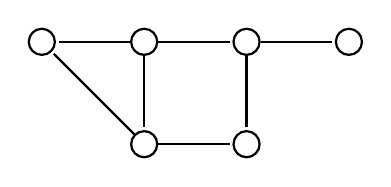
\begin{tikzpicture}[-,>=stealth,shorten >=1pt,auto,node distance=1.3cm, thick,main node/.style={scale=0.9,circle,draw,font=\sffamily\normalsize}]

            \node[circle, draw] (1) []{};
            \node[circle, draw] (2) [right of = 1]{};
            \node[circle, draw] (3) [below of = 1]{};
            \node[circle, draw] (4) [below of = 2]{};
            \node[circle, draw] (5) [left of = 1]{};
            \node[circle, draw] (6) [right of = 2]{};

            \draw[-] (1) to (2);
            \draw[-] (1) to (3);
            \draw[-] (2) to (4);
            \draw[-] (1) to (5);
            \draw[-] (3) to (4);
            \draw[-] (3) to (5);
            \draw[-] (2) to (6);

            ;
        \end{tikzpicture}
        % \caption{An example of a vertex cover.}
    \end{figure}

    is evaluated through the following ratio $$\rho(G) := \dfrac{\abs E}{\abs V} = \dfrac{7}{6} = 1.1 \overline 6$$ The problem that we are going to introduce is the following.

    \begin{frameddefn}{Densest Subgraph problem}
        The \tbf{Densest Subgraph} (DS) problem is defined as follows: given an undirected graph $G = (V, E)$, determine the induced subgraph of $G$ that maximizes its density. In other words, the problem asks to find a set of vertices $S^*$ in $$S^* \in \argmax_{S \subseteq V}{\rho(G[S])}$$
    \end{frameddefn}

    \begin{figure}[H]
        \centering
        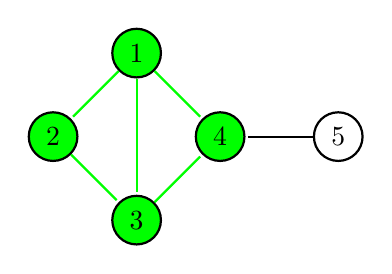
\begin{tikzpicture}[-,>=stealth,shorten >=1pt,auto,node distance=1.5cm, thick,main node/.style={scale=0.9,circle,draw,font=\sffamily\normalsize}]

            \node[circle, draw, fill=green] (1) []{1};
            \node[circle, draw, fill=green] (2) [below left of = 1]{2};
            \node[circle, draw, fill=green] (3) [below right of = 2]{3};
            \node[circle, draw, fill=green] (4) [below right of = 1]{4};
            \node[circle, draw] (5) [right of = 4]{5};

            \draw[-] (1) [green] to (2);
            \draw[-] (2) [green] to (3);
            \draw[-] (3) [green] to (4);
            \draw[-] (1) [green] to (4);
            \draw[-] (1) [green] to (3);
            \draw[-] (5) to (4);

            ;
        \end{tikzpicture}
        \caption{For instance, in this graph the set $S$ that maximizes $\rho(G[S])$ is given by $S = \{1, 2, 3, 4\}$, which yields a density of $\tfrac{5}{4} = 1.25$.}
    \end{figure}

    The densest subgraph is relevant because it actually \tit{maximizes} the average degree of its vertices. In fact, thanks to the handshaking lemma we have that $$\rho(G[S]) := \dfrac{\abs{E(G[S])}}{\abs S} = \dfrac{1}{2} \cdot \dfrac{2 \cdot \abs{E(G[S])}}{\abs s} = \dfrac{1}{2} \cdot \dfrac{\sum_{v \in S}{\deg (v)}}{\abs S} = \dfrac{1}{2} \avg_{v \in S}{\deg(v)}$$

    The LP that we will present which solves this problem is the following. However, to show that this LP actually yields a solution for DS is not trivial, and it will be proven through the following theorems.

    \begin{figure}[H]
        \centering
        \[\begin{array}{ccl}
            \qquad\qquad\quad
            & \max \; \displaystyle \sum_{e \in E} {x_e} \\\\
            & x_{ij} \le y_i & \forall i j \in E \\
            & x_{ij} \le y_j & \forall i j \in E \\
            & \sum\limits_{i \in V}{y_i} \le 1 \\
            & x_{ij} \ge 0 & \forall i j \in E \\
            & y_i \ge 0 & \forall i \in V \\
        \end{array}\]
        \caption{LP for DS.}
    \end{figure}

    \begin{framedlem}{}
        Given a graph $G = (V, E)$, for any $S \subseteq V$ there exists a feasible solution $\{x_e, y_i\}_{e \in E, i \in V}$ to the LP having value at least $\rho(G[S])$.
    \end{framedlem}

    \begin{proof}
        Given a set $S \subseteq V$, construct the following solution:

        \begin{itemize}
            \item $\forall ij \in E \quad x_{ij} := \soe{ll}{\dfrac{1}{\abs S} & i, j \in S \\ 0 & i \notin S \lor j \notin S}$
            \item $\forall i \in V \quad y_i := \soe{ll}{\dfrac{1}{\abs S} & i \in S \\ 0 & i \in V - S}$
        \end{itemize}

        We observe that

        \begin{itemize}
            \item $ij \in E(G[S]) \implies i, j \in S \implies \soe{l}{x_{ij} = \dfrac{1}{\abs S} \\ y_i = y_j = \dfrac{1}{\abs S}} \implies x_ij \le y_i, y_j$
            \item $ij \notin E(G[S]) \implies i \notin S \lor j \notin S \implies x_{ij} = 0$, but since $y_i, y_j \ge 0$ for any $i, j \in V$ by definition, it holds that $x_{ij} \le y_i, y_j$
        \end{itemize}

        Additionally, notice that $$\sum_{i \in V}{y_i} = \sum_{i \in S}{y_i} + \sum_{i \in V - S}{y_i} = \abs S \cdot \dfrac{1}{\abs S} + \abs {V - S} \cdot 0 = 1 \le 1$$

        This proves that this is a feasible solution to the LP. Lastly, the value of this solution is simply given by $$\sum_{e \in E}{x_e} = \sum_{e \in E(G[S])}{e} + \sum_{e \notin E(G[S])}{x_e} = \abs{E(G[S])} \cdot \dfrac{1}{\abs S} + \abs{E - E(G [S])} \cdot 0 = \dfrac{\abs{E(G[S])}}{\abs S} =: \rho(G[S])$$
    \end{proof}

    In particular, this lemma proves that if $S^*$ is an optimal solution for DS on a graph $G$, then there is a solution to this LP such that $\mathrm{LP^*} \ge \rho(G[S^*])$. The next theorem will prove that $\mathrm{LP^*} \le \rho(G[S^*])$ holds as well, which implies that our LP does in fact produce an optimal solution to DS, and that $\mathrm{IG_{DS}} = 1$.

    \begin{framedthm}{}
        Given a graph $G = (V, E)$, for any $\{x_e, y_i\}_{e \in E, i \in V}$ feasible solution to the LP that has value $v$, there exists a set $S \subseteq V$ such that $\rho(G[S]) \ge v$.
    \end{framedthm}

    \begin{proof}
        Consider a feasible solution $\{x_e', y_i'\}_{e \in E, i \in V}$ of the LP, having value $v$. We will construct another solution to the LP $\{x_e, y_i\}_{e \in E, i \in V}$ starting from the previous solution, as follows:

        \begin{itemize}
            \item $\forall i \in V \quad y_i := y_i'$
            \item $\forall ij \in E \quad x_{ij} := \min(y_i, y_j)$
        \end{itemize}

        It is easy to see that this is a feasible solution to the LP, in fact $$\forall ij \in E \quad x_{ij} := \min(y_i, y_j) \le y_i, y_j$$ and additionally, by feasibility of $\{x_e', y_i'\}_{e \in E, i \in V}$, we have that $$\sum_{i \in V}{y_i} = \sum_{i \in V}{y_i'} \le 1$$ Furthermore, note that $$v = \sum_{e \in E}{x_e'} \le \sum_{e \in E}{\min(y_i', y_j')} = \sum_{e \in E}{\min(y_i, y_j)} = \sum_{e \in E}{x_e}$$ meaning that the value of this solution is at least $v$, but it may be better --- this happens if $x_{ij} < y_i$ or $x_{ij} < y_j$ for some $ij \in E$, and if this is the case we say that there is some \tit{slack}.

        Next, we will construct a series of sets of vertices starting from this new LP solution we just defined. In particular, given a value $r \ge 0$, let $$S(r) := \{i \mid y_i \ge r\}$$ $$E(r) := \{e \mid x_e \ge r\}$$ Notice that $ij \in E(r) \iff i, j \in S(r)$, because $$ij \in E(r) \iff x_{ij} \ge r \iff \min(y_i, y_j) \ge r \iff y_i, y_j \ge r \iff i,j \in S(r)$$ which means that $S(r)$ and $E(r)$ are well-defined --- note that $E(G[S(r)]) = E(r)$.

        \claim{
            There exists a value $r^* \ge 0$ such that $\rho(G[S(r^*)]) \ge v$.
        }{
            Consider the solution $\{x_e, y_i\}_{e \in E, i \in V}$ to the LP that we constructed previously, and let $\pi$ be the permutation of the $y_i$'s such that $$0 \le y_{\pi (1)} \le y_{\pi (2)} \le \ldots \le y_{\pi(n - 1)} \le y_{\pi (n)}$$ which means that $\pi$ defines a sorting of the $y_i$'s. Now, consider the possible values of $r \ge 0$, and what happens inside $S(r)$:

            \begin{itemize}
                \item for $r = 0$, by feasibility of our solution we have that $$S(r) = S(0) := \{i \mid y_i \ge 0\} \implies \abs{S(r)} = n$$
                \item notice that for any value $0 \le r \le y_{\pi (1)} \le \ldots \le y_{\pi (n)}$, the value of $\abs{S(r)}$ will still be $n$, by its definition
                \item however, if $0 \le y_{\pi (1)} < r \le \ldots \le y_{\pi (n)}$, then the vertex $\pi(1)$ will be the only verterx not contained in $S(r)$, therefore $\abs{S(r)} = n - 1$
            \end{itemize}

            Repeating the same argument for all the possible values of $r$, we obtain the following graph for $\abs{S(r)}$.

            \begin{figure}[H]
                \centering
                \begin{tikzpicture}[scale=0.7]
                    \draw[-stealth] (-0.5,0) -- (2,0) node[below]{$y_{\pi(1)}$} -- (4,0) node[below]{$y_{\pi(2)}$} -- (7,0) node[below]{$\cdots$} -- (10,0) node[below]{$y_{\pi(n - 2)}$} -- (12,0) node[below]{$y_{\pi(n - 1)}$} -- (14,0) node[below]{$y_{\pi(n)}$} -- (15,0) node[right]{$r$};
                    \draw[-stealth] (0,-0.5) -- (0,0) node[below left]{0} -- (0,1) node[left]{1} -- (0,2) node[left]{2} -- (0,3.5) node[left]{$\cdots$} -- (0,5) node[left]{$n - 1$} -- (0,6) node[left]{$n$} -- (0,7.5) node[above]{$\abs{S(r)}$};
                    \draw[thick, orange] (0,6) -- (2,6) -- (2,5) -- (4,5) -- (4, 4) -- (5,4);
                    \draw[dashed, orange] (5,4) -- (6,4);
                    \draw[dashed, orange] (9,3) -- (8,3);
                    \draw[thick, orange] (14,0) -- (14,1) -- (12,1) -- (12,2) -- (10,2) -- (10,3) -- (9,3);
                \end{tikzpicture}
            \end{figure}

            From this graph, it is easy to see that computing the integral of $\abs{S(r)}$ is trivial, because
            \begin{equation*}
                \begin{split}
                    \int_{0}^{y_{\pi(n)}}{\abs{S(r)} \, d r} &= \int_{0}^{y_{\pi(1)}}{\abs{S(r)} \, dr} + \int_{y_{\pi(1)}}^{y_{\pi(2)}}{\abs{S(r)} \, dr} + \ldots + \int_{y_{\pi(n -1)}}^{y_{\pi(n)}}{\abs{S(r)} \, dr} \\
                                                             &= \int_{0}^{y_{\pi(1)}}{n \, dr} + \int_{y_{\pi(1)}}^{y_{\pi(2)}}{(n - 1) \, dr} + \ldots + \int_{y_{\pi(n - 1)}}^{y_{\pi(n)}}{1 \, dr} \\
                                                             &= n \cdot (y_{\pi(1)} - 0) + (n - 1) \cdot(y_{\pi(2)} - y_{\pi(1)}) + \ldots + 1 \cdot (y_{\pi(n)} - y_{\pi(n - 1)}) \\
                                                             &= y_{\pi(1)} \cdot\sbk{n - (n - 1)} + y_{\pi(2)}\cdot \sbk{(n - 1) - (n - 2)} + \ldots + y_{\pi(n)}\cdot (1 - 0) \\
                                                             &= y_{\pi(1)} \cdot 1 + y_{\pi(2)} \cdot 1 + \ldots + y_{\pi(n)} \cdot 1 \\
                                                             &= \sum_{i = 1}^n{y_{\pi(i)}} \\
                                                             &= \sum_{i \in V}{y_i} \\
                                                             &\le 1 \quad\quad (\mathrm{by \ feasibility \ of \ the \ solution})
                \end{split}
            \end{equation*}

            By the same argument, we can derive that $$\int_0^{y_{\pi(n)}}{\abs{E(r)} \, dr} = \sum_{e \in E}{x_e} \ge v$$ Note that the last inequality was proved before the claim.

            Lastly, we will prove the statement of the claim by way of contradiction. In particular, suppose that for all $r \ge 0$ it holds that $\rho(G[S(r)]) < v$. We can rewrite this inequality as follows $$\rho(G[S(r)]) := \dfrac{\abs{E(r)}}{\abs{S(r)}} < v \iff \abs{E(r)} < v \cdot \abs{S(r)}$$ This inequality can be used to upper bound the integral of $\abs{E(r)}$ \tit{point-by-point}, i.e. $$v \le \int_0^{y_{\pi(n - 1)}}{\abs{E(r)} \, dr} < \int_0^{y_{\pi(n - 1)}}{v \cdot \abs{S(r)} \, dr} = v \cdot \int_0^{y_{\pi(n - 1)}}{\abs{S(r)} \, dr} \le v \cdot 1 = v$$ meaning that $v < v$ $\lightning$.
        }

        Finally, since we proved that $G[S(r)]$ is well-defined, and this claim proves that there exists an $r^*$ such that $\rho(G[S(r^*)]) \ge v$, the statement holds.
    \end{proof}

    \subsection{Duality in Linear Programming}

    As we discussed at the beginning of this section, the cost of solving an LP generally depends on the number of \tit{variables} and \tit{constraints} it has. In particular, the LP we presented for solving DS has a \tit{large} number of both, which means that while the cost remains \tit{polynomial}, the degree of the polynomial is too high, making this approach \tbf{impractical} for large graphs.

    Now, we are going to present a \tbf{greedy algorithm}, developed by \textcite{charikar} in 2000, and we will prove that this algorithm yields a 2-approximation of DS.

    \begin{framedalgo}{Charikar's algorithm}
        Given an undirected graph $G = (V, E)$, the algorithm returns a 2-approximation solution of DS on $G$. \\
        \hrule

        \quad
        \begin{algorithmic}[1]
            \Function{Charikar}{$G$}
                \State $S_0 := V(G)$
                \For{$i \in [n - 1]$}
                    \State $\displaystyle v_i \in \argmin_{v \in S_{i - 1}}{\deg_{G[S_{i - 1}]}(v)}$
                    \State $S_i := S_{i - 1} - \{v_i\}$
                \EndFor
                \State \textbf{return} $\displaystyle S^* \in \argmax_{i \in [0, n - 1]}{\rho(G[S_i])}$
            \EndFunction
        \end{algorithmic}
    \end{framedalgo}

    \idea{
        The algorithm construct a series $S_0, \ldots, S_n$ of sets of vertices, such that $\abs{S_i} = n - i$, and at each iteration the $i$-th vertex that gets removed from $G[S_{i - 1}]$ is the one having minimum degree. At the end, the algorithm returns the set $S^*$ that maximizes the density of $G[S^*]$.
    }

    TODO \todo{example of non optimality}

    To prove that this algorithm yields a 2-approximation, we are going to introduce some definitions first.

    \begin{frameddefn}{Orientation}
        Given an undirected graph $G = (V, E)$, an \tbf{orientation} of $G$ is a function $\func{\phi}{E}{V}$ that assigns to each edge $\{u, v\} \in E$ either $u$ or $v$.
    \end{frameddefn}

    Note that, by definition for any $e \in E$ it holds that $\phi(e) \in e$. For instance, given the following graph

    \begin{figure}[H]
        \centering
        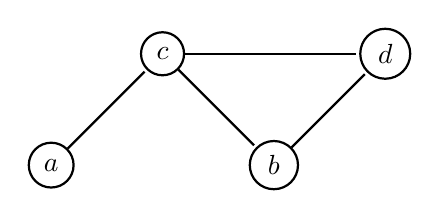
\begin{tikzpicture}[-,>=stealth,shorten >=1pt,auto,node distance=2cm, thick,main node/.style={scale=0.9,circle,draw,font=\sffamily\normalsize}]

            \node[circle, draw]  (1) []{$a$};
            \node[circle, draw]  (2) [above right of = 1]{$c$};
            \node[circle, draw]  (3) [below right of = 2]{$b$};
            \node[circle, draw]  (4) [above right of = 3]{$d$};

            % \path[every node/.style={font=\sffamily\small}]

            \draw[-] (1) to (2);
            \draw[-] (2) to (3);
            \draw[-] (2) to (4);
            \draw[-] (3) to (4);

            ;
        \end{tikzpicture}
        % \caption{Given the set of red vertices $S$, the green edges represent $\mathrm{cut}(S)$.}
    \end{figure}

    and the following function $\phi$

    \begin{center}
        \begin{tabular}{c|c c} 
             \hline
             $e$ & $\phi(e)$ \\
             \hline\hline
             $ac)$ & $c$ \\ 
             \hline
             $bc$ & $c$ \\
             \hline
             $bd$ & $b$ \\
             \hline
             $cd$ & $d$ \\
             \hline
        \end{tabular}
    \end{center}

    we would get the following orientation on $G$

    \begin{figure}[H]
        \centering
        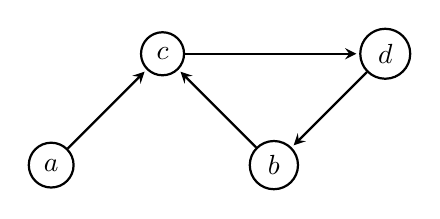
\begin{tikzpicture}[-,>=stealth,shorten >=1pt,auto,node distance=2cm, thick,main node/.style={scale=0.9,circle,draw,font=\sffamily\normalsize}]

            \node[circle, draw]  (1) []{$a$};
            \node[circle, draw]  (2) [above right of = 1]{$c$};
            \node[circle, draw]  (3) [below right of = 2]{$b$};
            \node[circle, draw]  (4) [above right of = 3]{$d$};

            % \path[every node/.style={font=\sffamily\small}]

            \draw[->] (1) to (2);
            \draw[->] (3) to (2);
            \draw[->] (2) to (4);
            \draw[->] (4) to (3);

            ;
        \end{tikzpicture}
        \caption{The previous graph, oriented through $\phi$.}
        \label{oriented graph}
    \end{figure}

    Given an orientation $\phi$ of $G$, and a vertex $v \in V(G)$ we will indicate with $\deg_\phi(v)$ the in-degree of $v$ w.r.t. $\phi$, i.e. $$\deg_\phi(v) := \abs{\{e \in E \mid \phi(e) = v\}}$$ For example, in the previous graph we have that $\deg_\phi(c) = 2$, $\deg_\phi(a) = 0$ and $\deg_\phi(b) = \deg_\phi(d) = 1$. By the same argument that proves the handshaking lemma, we observe that $$\sum_{v \in V(G)}{\deg_\phi(v)} = \abs E$$ Lastly, the maximum in-degree w.r.t. $\phi$ will be denoted as $$\Delta_\phi := \max_{v \in V} {\deg_\phi(v)}$$ We are now ready to prove the approximation ratio of Charikar's algorithm.

    \begin{framedthm}{\textsc{Charikar}'s approximation ratio}
        Given a graph $G$, and an optimal solution $\rho(G[S^*])$ for DS on $G$, let $M := \textsc{Charikar}(G)$; then, it holds that $\rho(G[S^*]) \le 2 M$.
    \end{framedthm}

    \begin{proof}
        We are going to prove this approximation ratio through two claims.

        \claim{
            Given an undirected graph $G$, and an optimal solution $\rho(G[S^*])$ for DS on $G$, for any orientation $\phi$ of $G$ it holds that $\rho(G[S^*]) \le \Delta_\phi$.
        }{
            By definition of $\phi$, each $uv \in E$ is going to be oriented towards either $u$ or $v$, therefore if $uv \in E(G[S^*])$ then $uv$ is going to be oriented towards a node of $S$. Hence, we have that \centeredeq{0.99}{$\displaystyle \abs{E(G[S^*])} \le \sum_{v \in V(G[S^*])}{\deg_\phi(v)} \le \sum_{v \in V(G[S^*])}{\Delta_\phi} = \abs {V[G(S^*)]} \cdot \Delta_\phi \iff \rho(G[S^*]) := \dfrac{\abs{E(G[S^*]})}{\abs{V(G[S^*])}} \le \Delta_\phi$}
        }

        Consider Charikar's algorithm; before proving the other claim, we need to introduce an orientation $\phi_\mathrm{GR}$ --- where GR stands for \tit{greedy} --- of $G$ defined as follows: if $v_i$ is the $i$-th vertex --- removed from $G[S_{i - 1}]$ --- picked by the algorithm, orient any edge $\{u, v_i\} \in E(G)$ towards $v_i$, for any $u \in V(G)$. For instance, Charikar's algorithm applied on the graph shown in \cref{oriented graph} would set $v_1 := a$, therefore $\phi(ca) = a$, and so on. This implies that $$\forall i \in [n] \quad \deg_{G[S_{i - 1}]}(v_i) = \deg_{\phi_\mathrm{GR}}(v_i)$$

        \claim{
            Given an undirected graph $G$, and $M := \textsc{Charikar}(G)$, it holds that $\Delta_{\phi_\mathrm{GR}} \le 2M$.
        }{
            Observe that for any $i \in [n]$ it holds that $$v_i \in \argmin_{v \in S_{i - 1}}{\deg_{G[S_{i - 1}]}(v)} \iff \deg_{G[S_{i - 1}]}(v_i) = \min_{v \in S_{i - 1}}{\deg_{G[S_{i - 1}]}(v)}$$ therefore, we have that 
            \begin{equation*}
                \begin{split}
                    \deg_{\phi_\mathrm{GR}}(v_i) &= \deg_{G[S_{i - 1}]}(v_i) \\
                                                 &= \min_{v \in S_{i - 1}}{\deg_{G[S_{i - 1}]}(v)} \\
                                                 &\le \avg_{v \in S_{i - 1}}{\deg_{G[S_{i - 1}]}(v)} \\
                                                 &= \displaystyle \dfrac{\sum_{v \in S_{i - 1}}{\deg_{G[S_{i - 1}]}(v)}}{\abs{S_{i - 1}}} \\
                                                 &= \dfrac{2 \abs{E(G[S_{i - 1}])}}{\abs{V(G[S_{i - 1}])}} \\
                                                 &=: 2\rho(G[S_{i - 1}])
                \end{split}
            \end{equation*}
            Finally, we get that
            \begin{equation*}
                \begin{split}
                    \Delta_{\phi_\mathrm{GR}} &:= \max_{v \in V(G)}{\deg_{\phi_\mathrm{GR}}(v)} \\
                                              &= \max_{i \in [n]}{\deg_{\phi_\mathrm{GR}}(v_i)} \\
                                              &\le \max_{i \in [n]}{2 \rho (G[S_{i - 1}])} \quad \quad (\mathrm{for \ the \ previous \ inequality}) \\
                                              &= 2 \max_{i \in [n]}{\rho(G[S_{i - 1}])} \\
                                              &\le 2 \max_{i \in [0, n - 1]}{\rho(G[S_i])} \\
                                              &=: 2M
                \end{split}
            \end{equation*}
        }

        Lastly, putting the two claims together, we get that for any optimal solution $\rho(G[S^*])$ of a given undirected graph $G$, if $M := \textsc{Charikar}(G)$ then $$\rho(G[S^*]) \le \Delta_{\phi_\mathrm{GR}} \le 2M$$
    \end{proof}

    In this proof, we defined $\phi_\mathrm{GR}$, which helped us determine the approximation ratio of the algorithm. But how did Charikar come up with such an orientation of the graph? To answer this question, we need to introduce the concept of the \tbf{duality} of linear programs.

    TODO \todo{da finire}

    \printbibliography % UNCOMMENT FOR BIBLIOGRAPHY

\end{document}
